\textbf{Nguyên lý Cực đại Entropy và Đàn chim Bay}

Vật lý hiện diện trong thế giới quanh ta, giúp mô tả các hành vi quần thể của những hệ thống tương tác phức tạp, từ đám khí lý tưởng đến đám đông người. Trong bài tập này, chúng ta sẽ cùng khám phá xem nguyên lý cực đại entropy đã được áp dụng như thế nào để thành lập lên một trong những lý thuyết Vật Lý Sinh thành công nhất hiện đại dùng để mô tả đàn chim bay (xem hình \ref{fig:Bird}A).

\begin{figure}[!h]
    \centering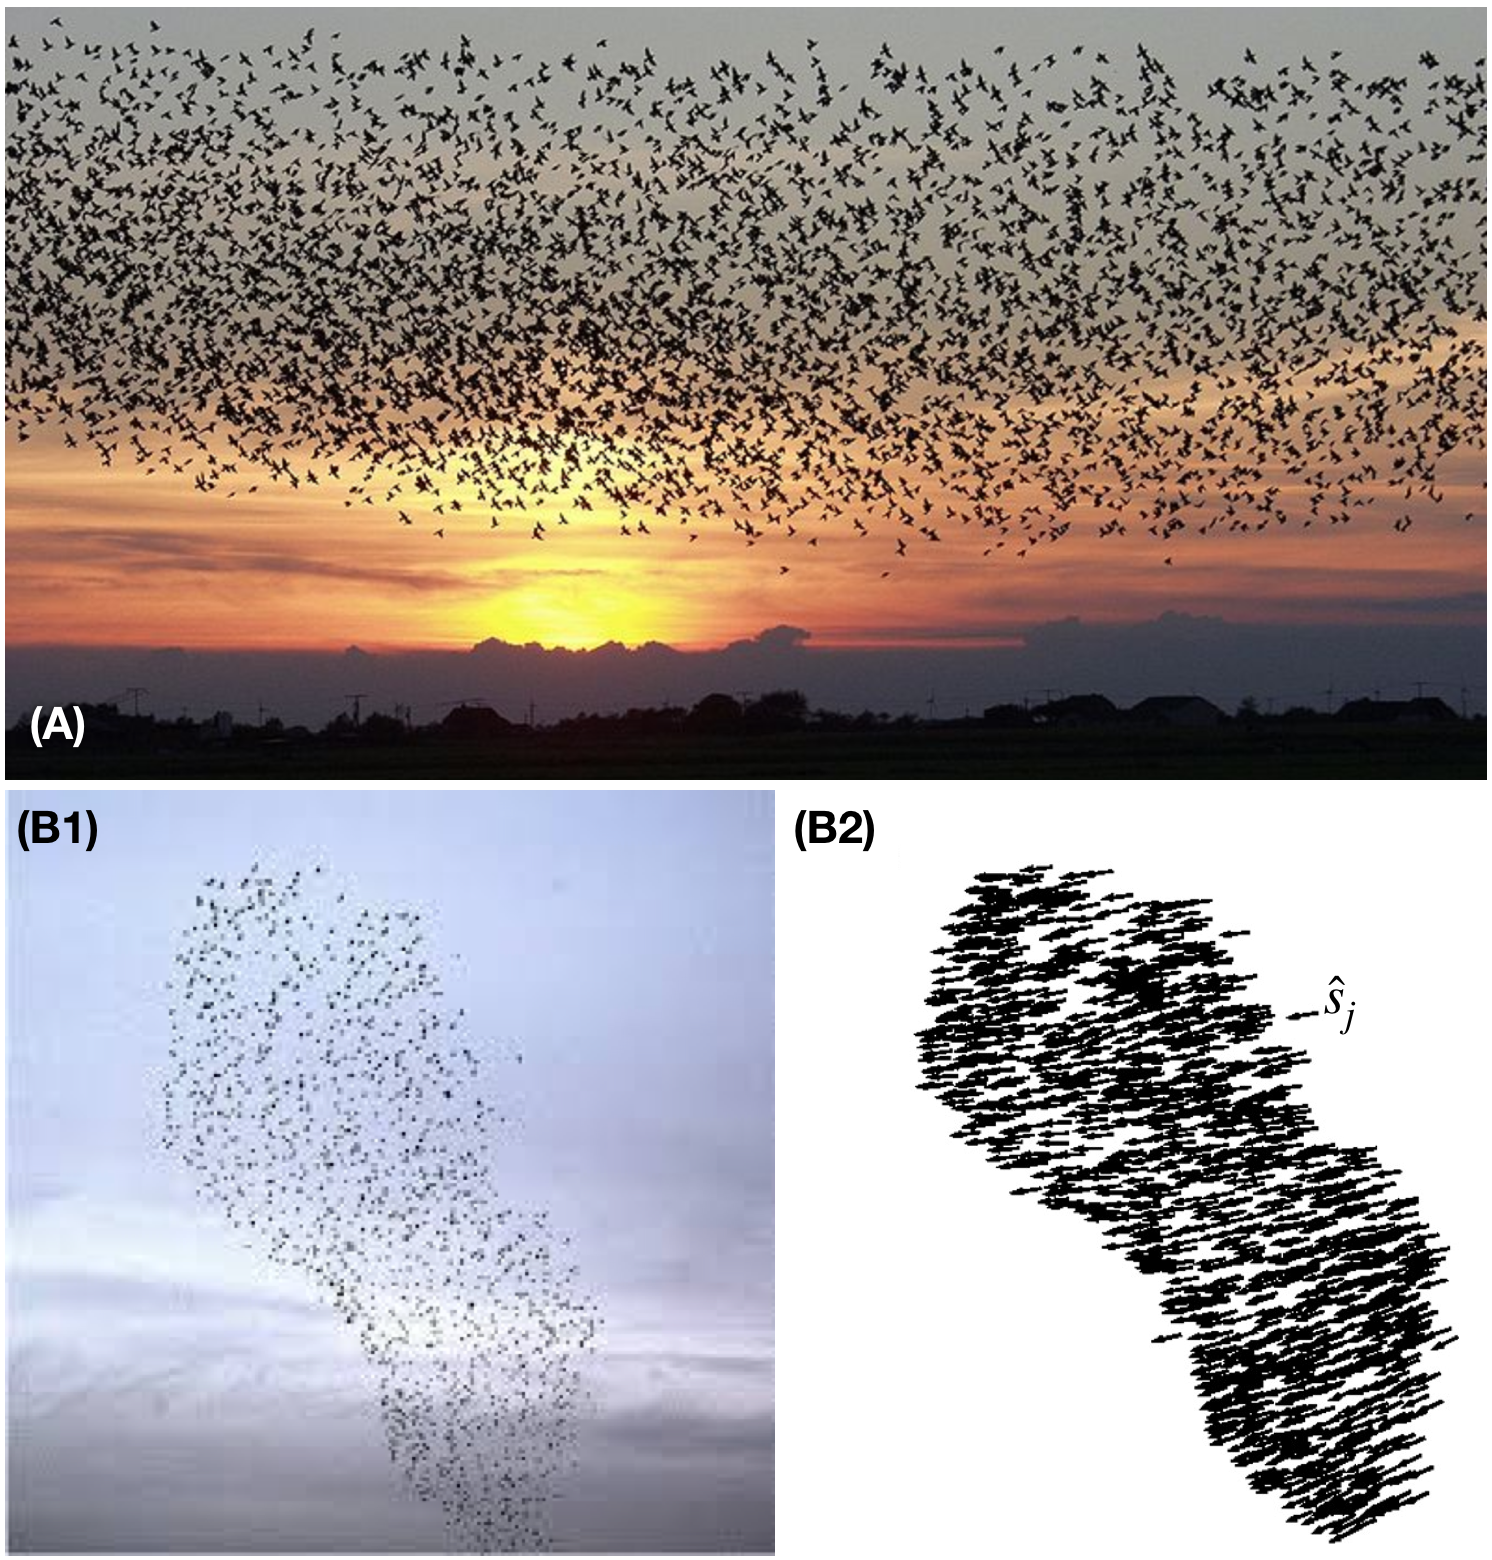
\includegraphics[width=0.96\textwidth]{Problem_5/Figs_P5/fig01.png}
    \caption{(A) Đàn chim bay. (B) Mô tả Toán học của một đàn chim bay, với (B1) là hình ảnh thô của đàn chim và (B2) là tập hợp các vector hướng bay của các cá thể trong đàn chim tại cùng thời điểm.}
    \label{fig:Bird}
\end{figure}

Nguyên lý cực đại entropy là một phương pháp thống kê dùng để suy ra phân phối xác suất không thiên vị nhất có thể dựa trên thông tin đã biết, đồng thời tránh đưa ra giả định về những điều chưa biết. Về cơ bản, nguyên lý này nói rằng, với một tập hợp các ràng buộc đã biết (như giá trị trung bình), phân phối xác suất tốt nhất là phân phối có entropy cao nhất mà vẫn thỏa mãn các ràng buộc này. Ở đây, công thức entropy thường được sử dụng là Boltzmann-Gibbs-Shannon entropy.

\ \ 

Với xác suất xảy ra của một đại lượng Vật Lý liên tục $X$, Boltzmann-Gibbs-Shannon entropy $S$ được xác định bởi giá trị trung bình của hàm \textit{độ ngạc nhiên} $I(x)=-\ln\left[ p(x)\right]$ theo biến $x$:
\begin{equation}
    S = \langle I \rangle = - \int_{\Omega_X} dx \ p(x) \ln\left[ p(x)\right] \ ,
\end{equation}
trong đó $x$ đại diện cho kết quả đo của đại lượng $X$, $p(x)$ là xác suất đo đại lượng $X$ cho ra kết quả $x$,  $\Omega_X$ là vùng khả dĩ của các kết quả đo cho đại lượng $X$.

\ \  

Chúng ta sẽ cùng nhau tìm hiểu về những ứng dụng của nguyên lý này trong việc diễn giải các kết quả thí nghiệm Vật lý, khi trong báo cáo chỉ cung cấp ít các thông tin liên quan.

\ \  

\textbf{1. Phương pháp nhân Lagrange}

Trước hết, chúng ta cùng nhau tìm hiểu về một phương pháp Toán học, vô cùng mạnh mẽ và hiệu quả, giúp chúng ta giải quyết các vấn đề tìm kiếm quỹ tích các điểm cực trị trong bối cảnh có ràng buộc -- phương pháp nhân Lagrange.

\ \ 

Xét việc tìm cực trị của hàm số $f(\vec{z})$ theo biến $\vec{z}\equiv [z_1, z_2, ..., z_{n_z}]$ (trong đó $n_z$ là số lượng các biến), với các điều kiện ràng buộc $C_k(\vec{z})$=0 (trong đó $k=1,2,...,n_C$, và $n_C$ là số lượng điều kiện ràng buộc). Hàm Lagrangian có thể được thiết lập như sau:
\begin{equation}
    L(\vec{Z}) = f(\vec{z}) - \sum_{k=1}^{n_C} \lambda_k C_k(\vec{z}) \ ,
\end{equation}
với biến $\vec{Z} \equiv [\vec{z}, \lambda_1, \lambda_2, \lambda_3, ..., \lambda_{n_C}]$.

\ \ 

\textbf{Câu hỏi a.} Hãy chứng minh rằng, điều kiện cực trị của hàm số $L(\vec{Z})$ theo biến $\vec{Z}$ có thể giúp chúng ta xác định được quỹ tích các điểm cực trị $\vec{z}$ của hàm số $f(\vec{z})$ dưới các ràng buộc $C_k(\vec{z})$.

\ \  

Những câu hỏi tiếp theo đây đều có thể được giải quyết sử dụng phương pháp nhân Lagrange.

\ \  

\textbf{2. Các hàm phân bố nội suy}

Để tránh rườm rà, nhiều báo cáo kết quả thí nghiệm thường không cung cấp toàn bộ dữ liệu thô từ các phép đo, mà chỉ trình bày giá trị ước lượng tốt nhất cùng với độ phân tán của các kết quả, thể hiện qua giá trị trung bình và phương sai.

\ \  

Hãy xác định hàm phân bố nội suy $p(x)$ cho xác suất thu được kết quả $x$ khi đo đại lượng $X$ thỏa mãn nguyên lý cực đại entropy, khi chúng ta chỉ biết những tính chất sau đây:

\ \  

\textbf{Câu hỏi b.} Vùng khả dĩ $\Omega_X$ là miền số thực i.e. $x\in (-\infty,\infty)$, giá trị đo trung bình của $X$ là $\mu$ và giá trị phương sai của $X$ là $\sigma^2 > 0$. Biểu diễn $p(x)$ theo $\mu$, $\sigma^2$, và biến $x$.

\ \  

\textbf{Câu hỏi c.} Vùng khả dĩ $\Omega_X$ là miền số dương i.e. $x\in[0,\infty)$, và giá trị đo trung bình của $X$ là $\mu$ (với $\mu > 0$). Biểu diễn $p(x)$ theo $\mu$ và biến $x$.

\ \  

Bây giờ, chúng ta sẽ áp dụng những kiến thức này vào một hệ vật lý cụ thể. Xét một quần thể gồm nhiều bậc tự do khác nhau mang năng lượng, e.g. một đám khí lý tưởng được cấu tạo từ nhiều phân tử khí khác nhau. Chúng ta sẽ tìm hiểu về tính chất thống kê của kết quả $\mathcal{E}$ khi đo giá trị năng lượng $E$ trên mỗi bậc tự do này.

\ \  

\textbf{Câu hỏi d.} Vùng khả dĩ $\Omega_E$ là miền chặn dưới i.e. $x\in[\mathcal{E}_{\min},\infty)$, và giá trị đo trung bình của $E$ là $\mathcal{E}_0$ (với $\mathcal{E}_0 > \mathcal{E}_{\min}$). Hãy chứng minh rằng, xác suất $p(\mathcal{E})$ -- cho kết quả $\mathcal{E}$ khi đo đại lượng $E$ -- thỏa mãn nguyên lý cực đại entropy chính là hàm phân bố Maxwell-Boltzmann:
\begin{equation}
    p(\mathcal{E}) \propto \exp\left( -\beta \mathcal{E} \right) \ \ ,
\end{equation}
trong đó $\beta$ là một hằng số nào đó liên hệ trực tiếp với $\mathcal{E}_0$.

\ \  

\textbf{3. Vật Lý Sinh mô tả đàn chim bay}

Có lẽ các bạn đã biết, hàm phân bố Maxwell-Boltzmann tạo ra cầu nối giữa hành vi ở cấp độ cá nhân và hành vi ở cấp độ quần thể, đặc biệt hiệu quả khi áp dụng cho những hệ Vật Lý được cấu tạo từ các cá thể đơn giản và vô tri. Tuy nhiên, với các hệ Vật Lý thường thấy trong thế giới Sinh học, nơi các cá thể có khả năng quan sát, xử lý thông tin và ra quyết định, để xây dựng cầu nối này thì hàm phân bố cần được sử dụng sẽ phải rất khác biệt.

\ \  

Xét một đàn chim bay, với chú chim $j$ ở vị trí $\vec{r}_j(t)$ và đang bay với vận tốc $\vec{v}_j(t)=d\vec{r}_j(t)/dt$ ($t$ là thời điểm hiện tại). Hướng bay của chú chim này được xác định bởi
$\hat{s}_j(t) = \vec{v}_j(t)/\left| \vec{v}_j(t)\right|$ (xem các hình \ref{fig:Bird}B), trong đó $\left|\vec{\circ}\right|$ là giá trị độ dài của vector $\vec{\circ}$. Định nghĩa giá trị liên kết $C_{jk}$ giữa cặp chim $j$ và $k$ theo giá trị trung bình của tích vô hướng hướng bay $\hat{s}_j(t) \cdot \hat{s}_k(t)$ theo thời gian $t$. Khi $C_{jk}$ càng gần với $1$, thì có nghĩa rằng cặp chim này càng cố gắng bay cùng hướng với nhau hơn.

\ \ 

Giả sử đàn chim bao gồm $N\gg 1$ chú chim, thế thì $j=1,2,3,...,N$ và mỗi \textit{vi thái} $\Theta$ của hướng bay đàn chim này có thể được xác đinh bởi $N$ các giác trị véc-tơ:
$$ \Theta \equiv \left[ \hat{s}_1, \hat{s}_2, \hat{s}_3, ..., \hat{s}_N \right] \ .$$
Cho biết tập hợp giá trị tất cả các hàm liên kết hướng bay $\{ C_{ij} \}$, chúng ta muốn xác định xác suất $p(\Theta)$ ở thời điểm bất kỳ quan sát được đàn chim bay đang sở hữu \textit{vi thái} $\Theta$.

\ \ 

\textbf{Câu hỏi e.} Chứng minh rằng:
\begin{equation}
    p(\Theta) \propto \exp\left[ -\frac12 \sum^N_{j=1} \sum^N_{k=1} \beta_{jk} \left(\hat{s}_j \cdot \hat{s}_k \right) \right] \ ,
\end{equation}
với mỗi giá trị $\beta_{jk}$ có thể được xác định từ tập hợp tất cả các giá trị liên kết hướng bay $\{ C_{jk}\}$.

\ \ 

Chú ý rằng, để đơn giản hóa câu hỏi ở trên, chúng ta xét ràng buộc là tất cả các tất cả các giá trị liên kết $C_{jk}$. Các nhà Vật Lý Sinh sử dụng ít ràng buộc hơn (chỉ với các cặp chim \textit{đủ gần} nhau) nhưng chặt hơn (tất cả các giá trị liên kết này đều bằng nhau). Nói cách khác, khi khớp lý thuyết này với thực nghiệm, thì chỉ có đúng hai giá trị tự do là kích thước hàng xóm $n$ và giá trị liên kết trong nhóm hàng xóm $C$. Kích thước hàng xóm $n$ xác định nhóm hàng xóm \textit{đủ gần} với một chú chim. Cụ thể, chim $j$ được coi là \textit{đủ gần} chim $k$ nếu nó nằm trong số $n$ chim gần nhất quanh chim $k$. Ý nghĩa sinh học ở đây là mỗi con chim đưa ra quyết định dựa trên quan sát và tương tác với các chim trong nhóm hàng xóm của mình, tập trung vào các tương tác địa phương thay vì toàn bộ bầy. Mô hình đơn giản này mô tả rất tốt những hành vi quần thể của nhiều bầy đàn sinh vật di cư đồng bộ khác nhau, e.g. bầy chim sáo đá châu Âu (\textit{Sturnus vulgaris}, xem hình \ref{fig:Sturn}) với $n\approx 11$ và $C\approx 0.996$. 

\begin{figure}[!h]
    \centering
\includegraphics[width=0.6\textwidth]{Problem_5/Figs_P5/fig02.jpg}\caption{Một chú chim sáo đá châu Âu (\textit{Sturnus vulgaris}).}
    \label{fig:Sturn}
\end{figure}

\ \ 
